\documentclass{article}\usepackage[]{graphicx}\usepackage[]{color}
%% maxwidth is the original width if it is less than linewidth
%% otherwise use linewidth (to make sure the graphics do not exceed the margin)
\makeatletter
\def\maxwidth{ %
  \ifdim\Gin@nat@width>\linewidth
    \linewidth
  \else
    \Gin@nat@width
  \fi
}
\makeatother

\definecolor{fgcolor}{rgb}{0.345, 0.345, 0.345}
\newcommand{\hlnum}[1]{\textcolor[rgb]{0.686,0.059,0.569}{#1}}%
\newcommand{\hlstr}[1]{\textcolor[rgb]{0.192,0.494,0.8}{#1}}%
\newcommand{\hlcom}[1]{\textcolor[rgb]{0.678,0.584,0.686}{\textit{#1}}}%
\newcommand{\hlopt}[1]{\textcolor[rgb]{0,0,0}{#1}}%
\newcommand{\hlstd}[1]{\textcolor[rgb]{0.345,0.345,0.345}{#1}}%
\newcommand{\hlkwa}[1]{\textcolor[rgb]{0.161,0.373,0.58}{\textbf{#1}}}%
\newcommand{\hlkwb}[1]{\textcolor[rgb]{0.69,0.353,0.396}{#1}}%
\newcommand{\hlkwc}[1]{\textcolor[rgb]{0.333,0.667,0.333}{#1}}%
\newcommand{\hlkwd}[1]{\textcolor[rgb]{0.737,0.353,0.396}{\textbf{#1}}}%

\usepackage{framed}
\makeatletter
\newenvironment{kframe}{%
 \def\at@end@of@kframe{}%
 \ifinner\ifhmode%
  \def\at@end@of@kframe{\end{minipage}}%
  \begin{minipage}{\columnwidth}%
 \fi\fi%
 \def\FrameCommand##1{\hskip\@totalleftmargin \hskip-\fboxsep
 \colorbox{shadecolor}{##1}\hskip-\fboxsep
     % There is no \\@totalrightmargin, so:
     \hskip-\linewidth \hskip-\@totalleftmargin \hskip\columnwidth}%
 \MakeFramed {\advance\hsize-\width
   \@totalleftmargin\z@ \linewidth\hsize
   \@setminipage}}%
 {\par\unskip\endMakeFramed%
 \at@end@of@kframe}
\makeatother

\definecolor{shadecolor}{rgb}{.97, .97, .97}
\definecolor{messagecolor}{rgb}{0, 0, 0}
\definecolor{warningcolor}{rgb}{1, 0, 1}
\definecolor{errorcolor}{rgb}{1, 0, 0}
\newenvironment{knitrout}{}{} % an empty environment to be redefined in TeX

\usepackage{alltt}

\usepackage{amsmath, amsthm, amsfonts, xfrac}
\usepackage{hyperref}

\title{Pol Sci 630: Problem Set 2 Solutions - Properties of Random Variables}
\author{Prepared by: Anh Le (\href{mailto:anh.le@duke.edu}{anh.le@duke.edu})}
\date{Due Date for Grading: Friday, September 11, 2015, 10 AM (Beginning of Class)}
\IfFileExists{upquote.sty}{\usepackage{upquote}}{}
\begin{document}
\maketitle

\section*{1. Expected Value and Its Properties}

\subsection*{a.} (1/4 point) (DeGroot, p. 216) Suppose that one word is to be selected at random from the sentence `the girl put on her beautiful red hat`. If X denotes the number of letters in the word that is selected, what is the value of E(X)?

\textbf{Solution}

As the number of letters in a word, $X$ can take on following values: $x \in \{2, 3, 4, 9 \}$, with probability as follows:

\begin{align}
P(X = 2) &= \frac{1}{8} \qquad \text{(1 word (``on'') out of 8 words in the sentence)} \\
P(X = 3) &= \frac{5}{8} \\
P(X = 4) &= \frac{1}{8} \\
P(X = 9) &= \frac{1}{8}
\end{align}

Therefore,

$$E(X) = \sum_{all x_i} x_i P(X = x_i) = 3.75$$

\subsection*{b.} (2/4 point) (Degroot p. 216) Suppose that one letter is to be selected at random from
the 30 letters in the sentence given in Exercise 4. If Y
denotes the number of letters in the word in which the
selected letter appears, what is the value of E(Y)?

\textbf{Solution}

$Y$ can take on values $y \in \{2, 3, 4, 9 \}$ with probability as follows:

\begin{align}
P(Y = 2) &= \frac{2}{30} &\text{O,N} \\
P(Y = 3) &= \frac{15}{30} &\text{T,H,E, P,U,T, H,E,R, R,E,D, H,A,T} \\
P(Y = 4) &= \frac{4}{30} &\text{G,I,R,L} \\
P(Y = 9) &= \frac{9}{30} &\text{B,E,A,U,T,I,F,U,L}
\end{align}

Therefore,

$$E(Y) = \sum_{\text{all $y_i$}} y_i P(Y = y_i) = \frac{73}{15} = 4.867$$

\subsection*{c.} (1/4 point) (Degroot, p. 224) Suppose that three random variables $X_1$, $X_2$, $X_3$ are uniformly distributed on the interval [0, 1]. They are also independent. Determine the value of $E[(X_1 - 2X_2 + X_3)^2]$.

\textbf{Solution}

\begin{align}
&E[(X_1 - 2 X_2 + X_3)^2] = \\
&= E(X_1^2) + 4E(X_2^2) + E(X_3^2) - 4E(X_1X_2) + 2E(X_1X_3) - 4E(X_2X_3) \\
&= E(X_1^2) + 4E(X_2^2) + E(X_3^2) - 4E(X_1)E(X_2) + 2E(X_1)E(X_3) - 4E(X_2)E(X_3)
\end{align}

Since each $X_i$ is uniformly distributed on $[0, 1]$,
\begin{align}
E(X_i) &= \frac{1}{2} \\
E(X_i^2) &= \int_0^1 x^2 dx = \frac{1}{3} \qquad{\text{law of unconscious statistician}}
\end{align}

Note: Law of unconscious statistician $E[g(x)] = \int g(x)f(x) dx$. This is an important theorem because it allows us to work with any function of a variable, as long as we know the distribution of that variable.

Alternatively, a common trick to find $E(X^2)$ is:

\begin{align}
E(X^2) &= Var(X) + [E(X)]^2 \\
&= \frac{1}{12} - \frac{1}{4} = \frac{1}{3} \qquad{\text{look up variance of uniform variable}}
\end{align}

Plug everything back in, we have $E[(X_1 - 2 X_2 + X_3)^2] = \frac{1}{2}$

\section*{2. Variance and its properties}

For this problem, you can use the properties of expected value.

\subsection*{a.} (1/4 point) Prove that $Var(aX + b) = a^2 Var(X)$.

\textbf{Solution}

\begin{align}
Var(aX + b) &= E[(aX + b)^2] - (E[(aX + b)])^2 \\
&= E[a^2X^2 + 2abX + b^2] - a^2[E(X)]^2 - 2abE(X)- b^2 \\
&= a^2(E(X^2) - [E(X)]^2) \\
&= a^2 Var(X) \qed
\end{align}

\subsection*{b.} (2/4 point) Implement in \verb`R` two functions that calculates the variance of the sum of two variables in two ways. The first calculates \verb`Var(X + Y)`. The second calculates \verb`Var(X) + Var(Y) + 2Cov(X, Y)`.

You should use vectorized operation and check that two functions return the same result. You may not use R's built-in \verb`var()` and \verb`cov()` functions.

\textbf{Solution}

\begin{knitrout}
\definecolor{shadecolor}{rgb}{0.969, 0.969, 0.969}\color{fgcolor}\begin{kframe}
\begin{alltt}
\hlstd{sumVar1} \hlkwb{<-} \hlkwa{function}\hlstd{(}\hlkwc{X}\hlstd{,} \hlkwc{Y}\hlstd{) \{}
  \hlstd{Z} \hlkwb{<-} \hlstd{X} \hlopt{+} \hlstd{Y}
  \hlkwd{return}\hlstd{(}\hlkwd{sum}\hlstd{((Z} \hlopt{-} \hlkwd{mean}\hlstd{(Z))}\hlopt{**}\hlnum{2}\hlstd{)} \hlopt{/} \hlstd{(}\hlkwd{length}\hlstd{(Z)} \hlopt{-} \hlnum{1}\hlstd{))}
\hlstd{\}}

\hlstd{sumVar2} \hlkwb{<-} \hlkwa{function}\hlstd{(}\hlkwc{X}\hlstd{,} \hlkwc{Y}\hlstd{) \{}
  \hlstd{varX} \hlkwb{<-} \hlkwd{sum}\hlstd{((X} \hlopt{-} \hlkwd{mean}\hlstd{(X))}\hlopt{**}\hlnum{2}\hlstd{)} \hlopt{/} \hlstd{(}\hlkwd{length}\hlstd{(X)} \hlopt{-} \hlnum{1}\hlstd{)}
  \hlstd{varY} \hlkwb{<-} \hlkwd{sum}\hlstd{((Y} \hlopt{-} \hlkwd{mean}\hlstd{(Y))}\hlopt{**}\hlnum{2}\hlstd{)} \hlopt{/} \hlstd{(}\hlkwd{length}\hlstd{(Y)} \hlopt{-} \hlnum{1}\hlstd{)}
  \hlstd{covXY} \hlkwb{<-} \hlkwd{sum}\hlstd{((X} \hlopt{-} \hlkwd{mean}\hlstd{(X))} \hlopt{*} \hlstd{(Y} \hlopt{-} \hlkwd{mean}\hlstd{(Y)))} \hlopt{/} \hlstd{(}\hlkwd{length}\hlstd{(X)} \hlopt{-} \hlnum{1}\hlstd{)}
  \hlkwd{return}\hlstd{(varX} \hlopt{+} \hlstd{varY} \hlopt{+} \hlnum{2} \hlopt{*} \hlstd{covXY)}
\hlstd{\}}

\hlkwd{set.seed}\hlstd{(}\hlnum{1}\hlstd{)}
\hlstd{X} \hlkwb{<-} \hlkwd{rnorm}\hlstd{(}\hlnum{100}\hlstd{) ; Y} \hlkwb{<-} \hlkwd{rnorm}\hlstd{(}\hlnum{100}\hlstd{)}
\hlkwd{sumVar1}\hlstd{(X, Y)}
\end{alltt}
\begin{verbatim}
## [1] 1.722583
\end{verbatim}
\begin{alltt}
\hlkwd{sumVar2}\hlstd{(X, Y)}
\end{alltt}
\begin{verbatim}
## [1] 1.722583
\end{verbatim}
\end{kframe}
\end{knitrout}


\subsection*{c.} (1/4 point) (Degroot, p. 232) Suppose that one word is selected at random from the sentence `the girl put on her beautiful red hat`. If $X$ denotes the number of letters in the word that is selected, what is the value of $Var(X)$?

\textbf{Solution}

Notice that the distribution of $X$ is the same as in Question 1a), therefore $E(X) = 3.75$ and

$$E(X^2) = \sum_{\text{all $x_i$}} x_i^2 P(X = x_i) = \frac{73}{4}$$

Thus,

\begin{align}
Var(X) &= E(X^2) - [E(X)]^2 = \frac{67}{16}
\end{align}

\section*{3. Binomial distribution}

(Credit to Jan) This problem is taken from Pitman (1993) Probability

Suppose a fair coin is tossed n times. Find a simple formula in terms of n and k for the following probability: $Pr(k\ heads | k-1\ heads\ or\ k\ heads)$. Please pay close attention to the formula, particularly what event is conditioned on what events. (Ch. 2.1, Problem 10 b) (p. 91)

Hint 1: Use the binomial distribution to model this.

Hint 2: Use $Pr(A | B) = \dfrac{Pr (A \cap B)}{Pr (B)}$ with $A = k\ heads$ and $B = k-1\ heads\ or\ k\ heads)$

\textbf{Solution (Credit to Jan)}

$Pr(k\ heads | k-1\ heads\ or\ k\ heads)$
$\\= \dfrac{Pr(k\ heads \cap (k-1\ heads\ or\ k\ heads) )}{Pr (k\ heads) + Pr (k-1\ heads)}$
$\\= \dfrac{Pr(k\ heads)}{Pr (k\ heads) + Pr (k-1\ heads)}$
$\\ = \dfrac{\binom{n}{k}0.5^k0.5^{n-k}}{\binom{n}{k}0.5^k0.5^{n-k} + \binom{n}{k-1}0.5^{k-1}0.5^{n-(k-1)}}$
$\\ = \dfrac{\binom{n}{k}0.5^n}{\binom{n}{k}0.5^n + \binom{n}{k-1}0.5^n}$
$ \\ = \dfrac{\binom{n}{k}}{\binom{n}{k} + \binom{n}{k-1}}$
$\\ = \dfrac{\dfrac{n!}{(n-k)! k!}}{\dfrac{n!}{(n-k)! k!} + \dfrac{n!}{(n-(k-1))! (k-1)!}}$
$\\ = \dfrac{\dfrac{n!}{(n-k)! k!} * \dfrac{n-k+1}{n-k+1}}{\dfrac{n!}{(n-k)! k!} * \dfrac{n-k+1}{n-k+1} + \dfrac{n!}{(n-k+1)! (k-1)!}*\dfrac{k}{k}}$
$\\ = \dfrac{\dfrac{n!(n-k+1)}{(n-k+1)! k!}}{\dfrac{n!(n-k+1)}{(n-k+1)! k!} + \dfrac{n!}{(n-k+1)! k!}}$
$\\ = \dfrac{n!(n-k+1)}{n!(n-k+1)+n!k}$
$\\ = \dfrac{n-k+1}{n-k+1+k}$
$\\= \dfrac{n-k+1}{n+1}$

\section*{4. Plotting distribution}

For this problem, you'll need to Google some R techniques (e.g. side-by-side / overlapping plot). Also, label the axes and the plots accordingly.

\subsection*{a.} (1/4 point) Download a variable you are interested in, using \verb`WDI`. Plot the histogram, density plot, boxplot, and normal quantile plot.

\begin{knitrout}
\definecolor{shadecolor}{rgb}{0.969, 0.969, 0.969}\color{fgcolor}\begin{kframe}
\begin{alltt}
\hlcom{# install.packages("WDI")}
\hlkwd{library}\hlstd{(WDI)}
\end{alltt}


{\ttfamily\noindent\itshape\color{messagecolor}{\#\# Loading required package: RJSONIO}}\begin{alltt}
\hlstd{d_land} \hlkwb{<-} \hlkwd{WDI}\hlstd{(}\hlkwc{indicator} \hlstd{=} \hlkwd{c}\hlstd{(}\hlstr{"AG.LND.ARBL.ZS"}\hlstd{,} \hlstr{"NY.GDP.PCAP.KD"}\hlstd{),}
              \hlkwc{start}\hlstd{=}\hlnum{2010}\hlstd{,} \hlkwc{end}\hlstd{=}\hlnum{2010}\hlstd{,} \hlkwc{extra}\hlstd{=}\hlnum{TRUE}\hlstd{)}
\hlstd{d_land} \hlkwb{<-} \hlstd{d_land[d_land}\hlopt{$}\hlstd{region} \hlopt{!=} \hlstr{"Aggregates"}\hlstd{, ]}

\hlcom{# Rename column}
\hlkwd{colnames}\hlstd{(d_land)[}\hlkwd{colnames}\hlstd{(d_land)} \hlopt{==} \hlstr{"AG.LND.ARBL.ZS"}\hlstd{]} \hlkwb{<-} \hlstr{"arable_land_pct"}
\hlkwd{colnames}\hlstd{(d_land)[}\hlkwd{colnames}\hlstd{(d_land)} \hlopt{==} \hlstr{"NY.GDP.PCAP.KD"}\hlstd{]} \hlkwb{<-} \hlstr{"gdp_percapita"}

\hlstd{xlabel} \hlkwb{<-} \hlstr{"Arable land as % of total land"}
\hlkwd{par}\hlstd{(}\hlkwc{mfrow}\hlstd{=}\hlkwd{c}\hlstd{(}\hlnum{2}\hlstd{,} \hlnum{2}\hlstd{))}
\hlkwd{hist}\hlstd{(d_land}\hlopt{$}\hlstd{arable_land_pct,} \hlkwc{main} \hlstd{=} \hlstr{"Histogram"}\hlstd{,} \hlkwc{xlab} \hlstd{= xlabel)}
\hlkwd{plot}\hlstd{(}\hlkwd{density}\hlstd{(d_land}\hlopt{$}\hlstd{arable_land_pct,} \hlkwc{na.rm} \hlstd{=} \hlnum{TRUE}\hlstd{),} \hlkwc{main} \hlstd{=} \hlstr{"Density plot"}\hlstd{,} \hlkwc{xlab} \hlstd{= xlabel)}
\hlkwd{boxplot}\hlstd{(d_land}\hlopt{$}\hlstd{arable_land_pct,} \hlkwc{main} \hlstd{=} \hlstr{"Box plot of arable land"}\hlstd{)}
\hlkwd{qqnorm}\hlstd{(d_land}\hlopt{$}\hlstd{arable_land_pct,} \hlkwc{main} \hlstd{=} \hlstr{"Normal Q-Q plot of arable land"}\hlstd{)}
\hlkwd{qqline}\hlstd{(d_land}\hlopt{$}\hlstd{arable_land_pct)}
\end{alltt}
\end{kframe}
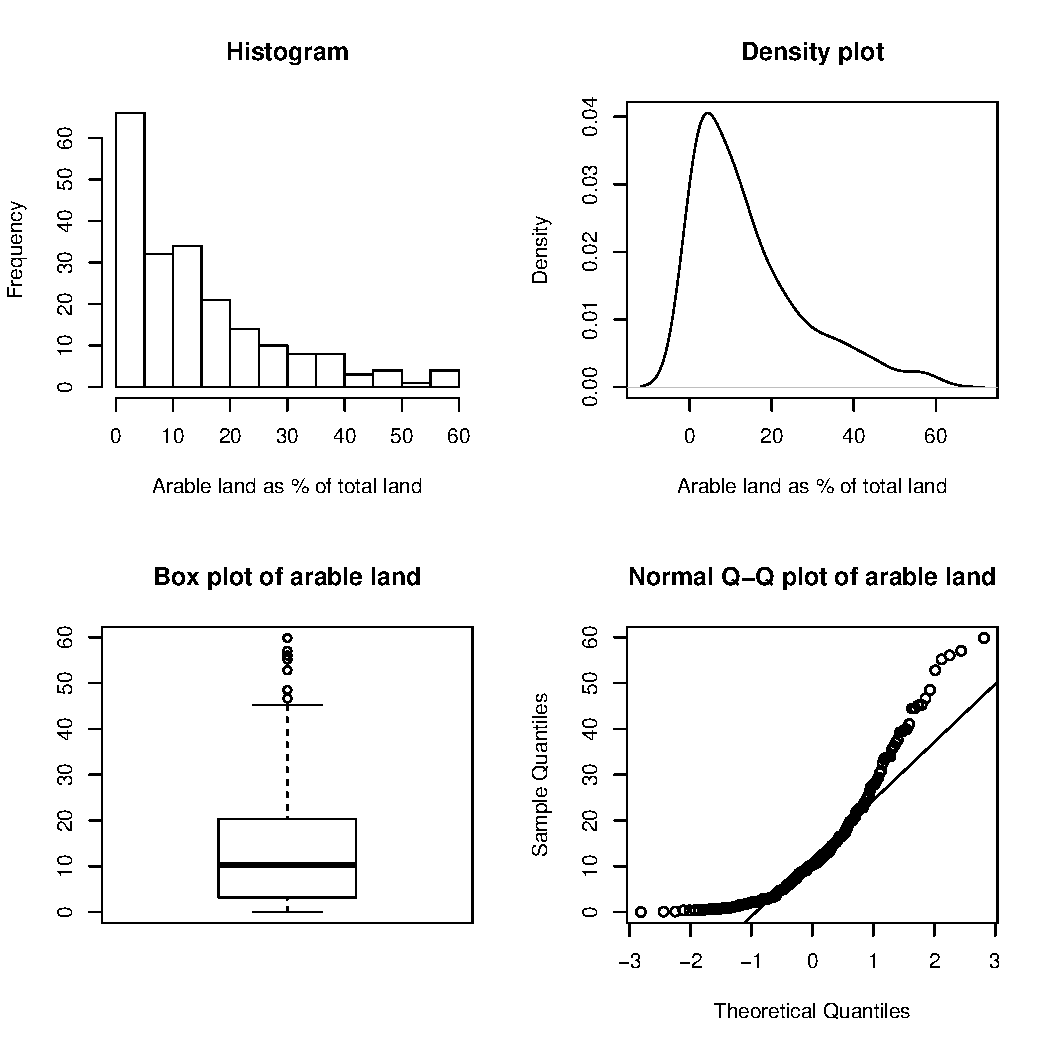
\includegraphics[width=\maxwidth]{figure/4a-1} 

\end{knitrout}


\subsection*{b.} (1/4 point) Plot the density plots of that variable for Europe and Asia, 1) side by side (Hint: \verb`par(mfrow=c(?, ?))`), and 2) overlapping in the same plot.

\begin{knitrout}
\definecolor{shadecolor}{rgb}{0.969, 0.969, 0.969}\color{fgcolor}\begin{kframe}
\begin{alltt}
\hlkwd{par}\hlstd{(}\hlkwc{mfrow}\hlstd{=}\hlkwd{c}\hlstd{(}\hlnum{1}\hlstd{,} \hlnum{3}\hlstd{))}
\hlstd{europe_density} \hlkwb{<-} \hlkwd{density}\hlstd{(}
  \hlstd{d_land[d_land}\hlopt{$}\hlstd{region} \hlopt{==} \hlstr{"Europe & Central Asia (all income levels)"}\hlstd{,} \hlstr{"arable_land_pct"}\hlstd{],}
  \hlkwc{na.rm}\hlstd{=}\hlnum{TRUE}\hlstd{)}
\hlstd{asia_density} \hlkwb{<-} \hlkwd{density}\hlstd{(}
  \hlstd{d_land[d_land}\hlopt{$}\hlstd{region} \hlopt{==} \hlstr{"East Asia & Pacific (all income levels)"}\hlstd{,} \hlstr{"arable_land_pct"}\hlstd{],}
  \hlkwc{na.rm}\hlstd{=}\hlnum{TRUE}\hlstd{)}
\hlkwd{plot}\hlstd{(europe_density,} \hlkwc{main} \hlstd{=} \hlstr{"Arable land (Europe)"}\hlstd{)}
\hlkwd{plot}\hlstd{(asia_density,} \hlkwc{main} \hlstd{=} \hlstr{"Arable land (Asia)"}\hlstd{)}

\hlcom{# Overlaying}
\hlkwd{plot}\hlstd{(asia_density,} \hlkwc{xlim} \hlstd{=} \hlkwd{c}\hlstd{(}\hlopt{-}\hlnum{20}\hlstd{,} \hlnum{80}\hlstd{),} \hlkwc{col}\hlstd{=}\hlstr{'red'}\hlstd{,} \hlkwc{main} \hlstd{=} \hlstr{"Asia and Europe"}\hlstd{)}
\hlkwd{lines}\hlstd{(europe_density,} \hlkwc{col}\hlstd{=}\hlstr{'blue'}\hlstd{)}
\hlkwd{legend}\hlstd{(}\hlnum{25}\hlstd{,} \hlnum{.05}\hlstd{,} \hlkwd{c}\hlstd{(}\hlstr{"Asia"}\hlstd{,} \hlstr{"Europe"}\hlstd{),}
  \hlkwc{lty}\hlstd{=}\hlkwd{c}\hlstd{(}\hlnum{1}\hlstd{,}\hlnum{1}\hlstd{),} \hlcom{# gives the legend appropriate symbols (lines)}
  \hlkwc{lwd}\hlstd{=}\hlkwd{c}\hlstd{(}\hlnum{1}\hlstd{,}\hlnum{1}\hlstd{),}\hlkwc{col}\hlstd{=}\hlkwd{c}\hlstd{(}\hlstr{"red"}\hlstd{,}\hlstr{"blue"}\hlstd{))}
\end{alltt}
\end{kframe}
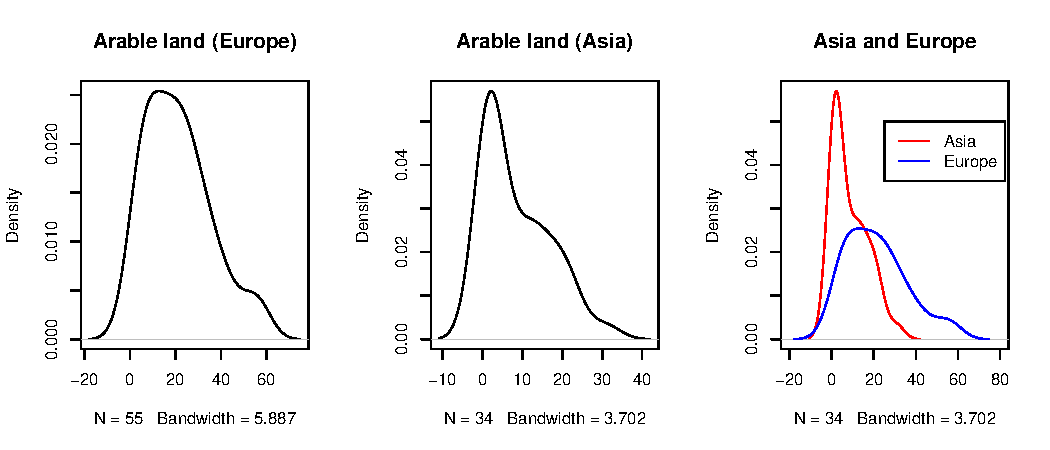
\includegraphics[width=\maxwidth]{figure/4b-1} 
\begin{kframe}\begin{alltt}
\hlcom{# Tutorial for legend: http://www.r-bloggers.com/adding-a-legend-to-a-plot/}
\end{alltt}
\end{kframe}
\end{knitrout}

\subsection*{c.} (1/4 point) Draw the scatterplot of that variable against another variable.

\begin{knitrout}
\definecolor{shadecolor}{rgb}{0.969, 0.969, 0.969}\color{fgcolor}\begin{kframe}
\begin{alltt}
\hlkwd{plot}\hlstd{(d_land}\hlopt{$}\hlstd{arable_land_pct,} \hlkwd{log}\hlstd{(d_land}\hlopt{$}\hlstd{gdp_percapita),}
     \hlkwc{xlab} \hlstd{=} \hlstr{"Arable land as % of total land"}\hlstd{,}
     \hlkwc{ylab} \hlstd{=} \hlstr{"log GDP per capita (2005 USD)"}\hlstd{,}
     \hlkwc{main} \hlstd{=} \hlstr{"Arable land and GDP per capita"}\hlstd{)}
\end{alltt}
\end{kframe}
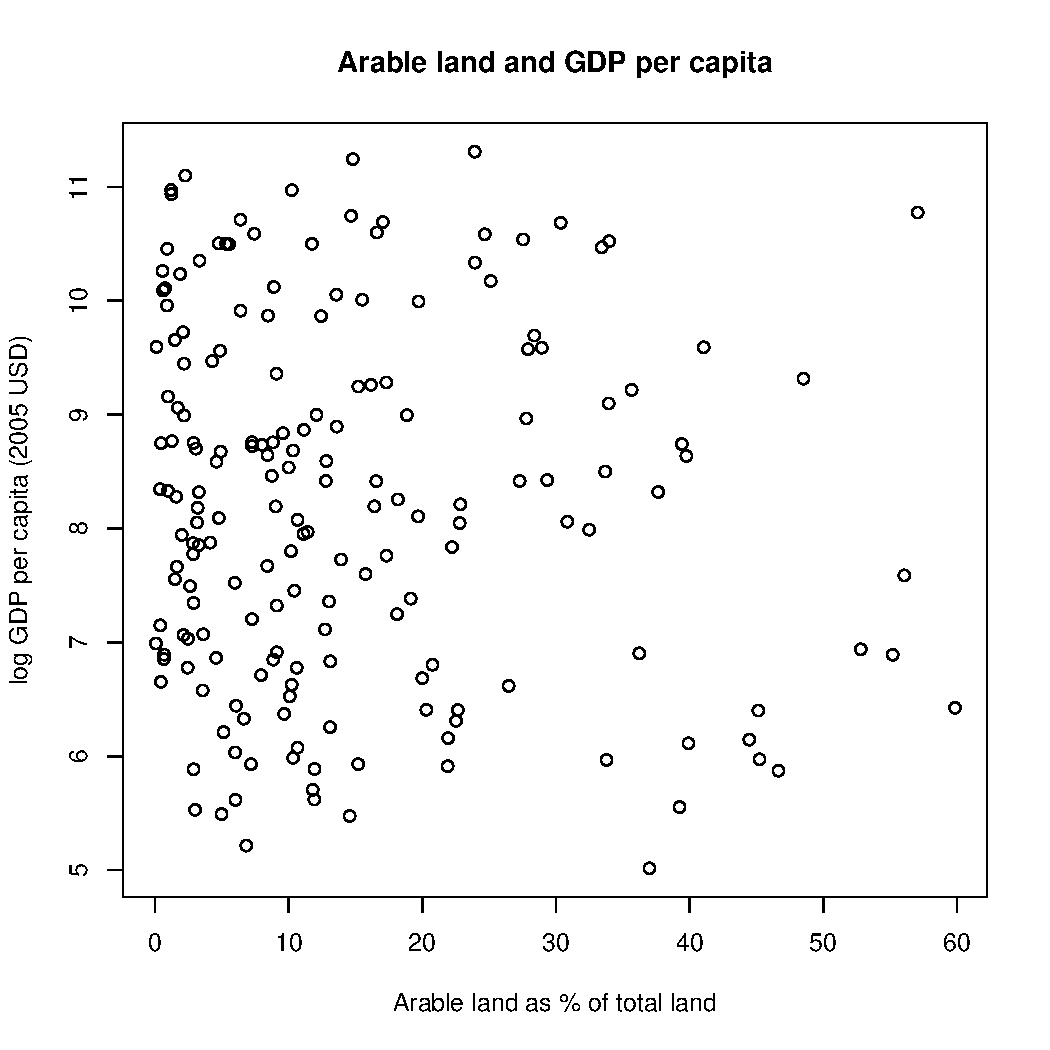
\includegraphics[width=\maxwidth]{figure/unnamed-chunk-1-1} 

\end{knitrout}


\subsection*{d.} (1/4 point) Label the point that represents your country (Hint: \href{https://chemicalstatistician.wordpress.com/2013/03/02/adding-labels-to-points-in-a-scatter-plot-in-r/}{Tutorial}) and color it red (Some Googling involved)

\begin{knitrout}
\definecolor{shadecolor}{rgb}{0.969, 0.969, 0.969}\color{fgcolor}\begin{kframe}
\begin{alltt}
\hlkwd{par}\hlstd{(}\hlkwc{mfrow}\hlstd{=}\hlkwd{c}\hlstd{(}\hlnum{1}\hlstd{,} \hlnum{1}\hlstd{))}
\hlkwd{plot}\hlstd{(}\hlkwd{log}\hlstd{(gdp_percapita)} \hlopt{~} \hlstd{arable_land_pct,}
     \hlkwc{data} \hlstd{= d_land,}
     \hlkwc{xlab} \hlstd{=} \hlstr{"Arable land as % of total land"}\hlstd{,}
     \hlkwc{ylab} \hlstd{=} \hlstr{"log GDP per capita (2005 USD)"}\hlstd{,}
     \hlkwc{main} \hlstd{=} \hlstr{"Arable land and GDP per capita"}\hlstd{)}
\hlstd{d_land_Vietnam} \hlkwb{<-} \hlstd{d_land[d_land}\hlopt{$}\hlstd{country} \hlopt{==} \hlstr{"Vietnam"}\hlstd{, ]}
\hlkwd{with}\hlstd{(d_land_Vietnam,}
     \hlkwd{text}\hlstd{(}\hlkwd{log}\hlstd{(gdp_percapita)} \hlopt{~} \hlstd{arable_land_pct,} \hlkwc{labels} \hlstd{=} \hlstr{"Vietnam"}\hlstd{,}
          \hlkwc{pos} \hlstd{=} \hlnum{3}\hlstd{,} \hlkwc{col} \hlstd{=} \hlstr{'red'}\hlstd{))}
\hlkwd{points}\hlstd{(d_land_Vietnam}\hlopt{$}\hlstd{arable_land_pct,} \hlkwd{log}\hlstd{(d_land_Vietnam}\hlopt{$}\hlstd{gdp_percapita),}
       \hlkwc{pch} \hlstd{=} \hlnum{16}\hlstd{,} \hlkwc{col} \hlstd{=} \hlstr{'red'}\hlstd{)}
\end{alltt}
\end{kframe}
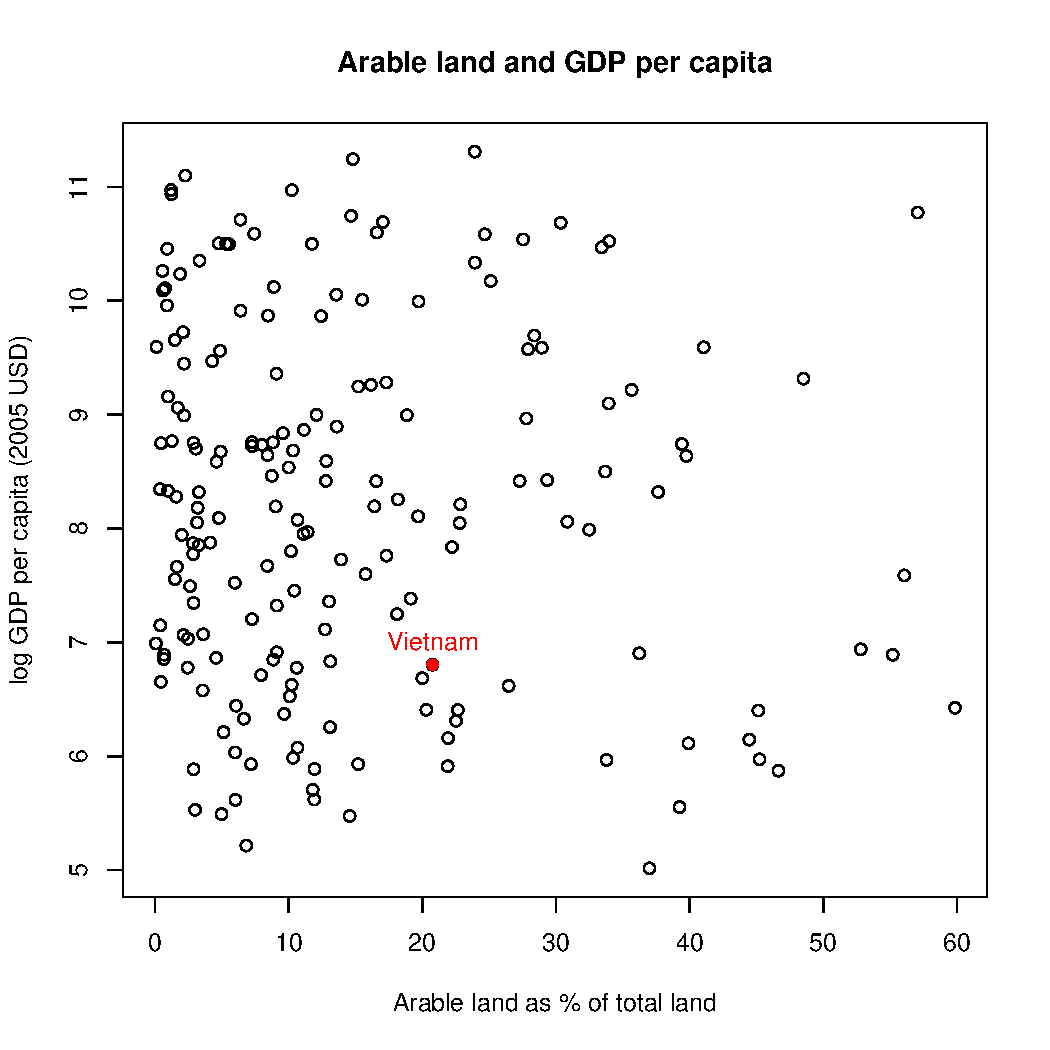
\includegraphics[width=\maxwidth]{figure/unnamed-chunk-2-1} 

\end{knitrout}

\end{document}
